Faulty cores are an unfortunate reality of \acp{MPSoC}. After some time, at least one core is likely to fail.
However, using hardware monitors, these faults can be reliably detected, sometimes even before the core actually starts failing~\cite{zhang2011dependability,zhao2019health}.
A strategy to deal with faulty cores, when detected, is to migrate tasks executing in that core to a different core.
This way, when the core fails, the execution can continue without the application failing. 

While such a remapping strategy is ideal for preserving the functional correctness of applications, it can have negative consequences on the performance of the application.
Especially for real-time applications, where the timing performance is part of the functionality, these consequences can be as fatal as a core failing without being detected or without remapping.
Moreover, in mixed-criticality domains, a pre-determined mapping can be varied at runtime due to priority issues or similar unforseen circumstances.
To deal with this, we propose to search for \emph{robust} mappings\index{robust mappings}~\cite{hempel_scopes17}.
We say a mapping is robust when its runtime properties are unchanged by minor variations in a mapping.

The robustness of a mapping and the corresponding methods proposed in this section are appropriate for soft or firm\footnote{recall that a firm real-time application is one where the computation and data is useless after missing a deadline, yet a small percentage of missed deadlines might still be tolerable} real-time applications, especially in mixed-criticality contexts.
In this context, we say a mapping is \emph{feasible} if its execution time is below a specified real-time deadline.
To test if a (feasible) mapping is robust, we apply \emph{perturbations}\index{mapping perturbations}.
A perturbation consists in taking the mapping and changing it partially, to see if it is (still) feasible.
A robust mapping should be resistant to perturbations, as motivated by the remapping scenarios described before.

To find such robust mappings we propose~\cite{hempel_scopes17} adapting the bio-inspired algorithm for called $L_p$-adaptation~\cite{asmus2017lp}.
This algorithm uses the metric space structure of the mapping space (cf. Section~\ref{sec:metric_spaces}) to navigate it and find a \emph{design center}.\index{design center}
For a fixed probability $P$, a design center is a feasible point $m$ in the design space, such that points in a neighborhood of $m$ are feasible with probability at least $P$.
For the context of this discussion, we consider neighborhoods of the form $B_r(m)$, a ball with radius $r$ around the point $m$.
The $L_p$-adaptation algorithm seeks to find and $m$ which maximizes the radius $r$ such that the $B_r(m)$ is feasible with probability at least $P$.

\begin{figure*}[t]
  \centering
	\begin{subfigure}[b]{0.33\textwidth}
    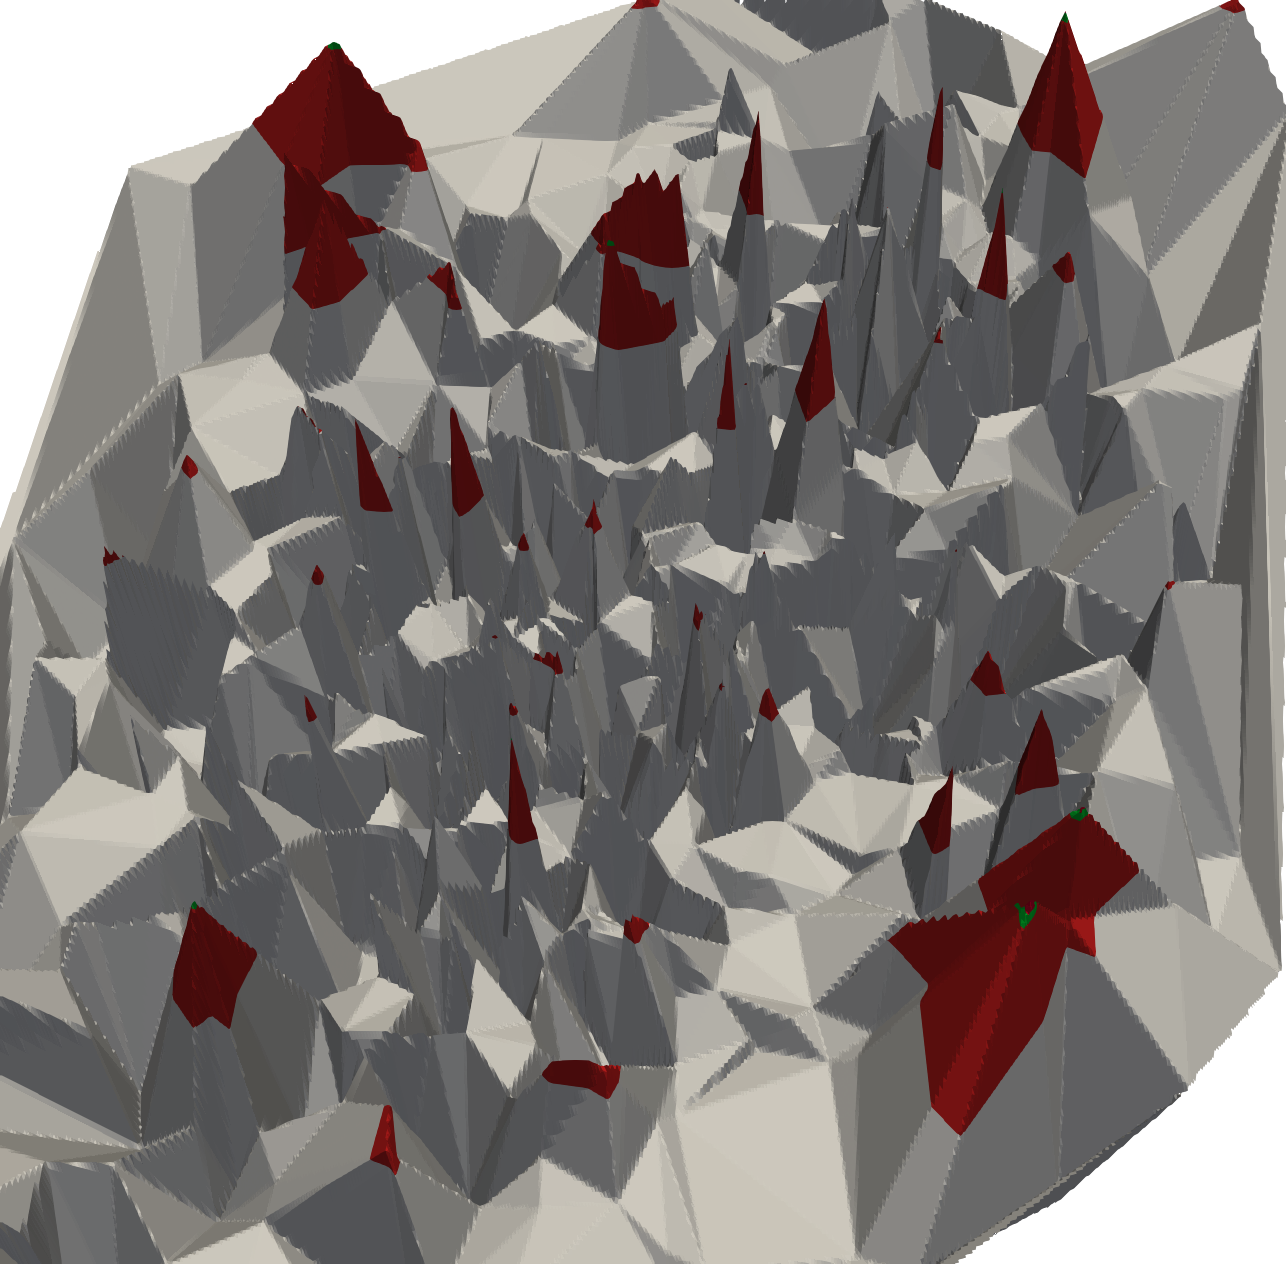
\includegraphics[width=\textwidth]{figures/coolidge-af-high-threshold.png}
		\caption{High threshold.}
		\label{fig:lvars-bench-cores}
	\end{subfigure}
	~
	\begin{subfigure}[b]{0.33\textwidth}
    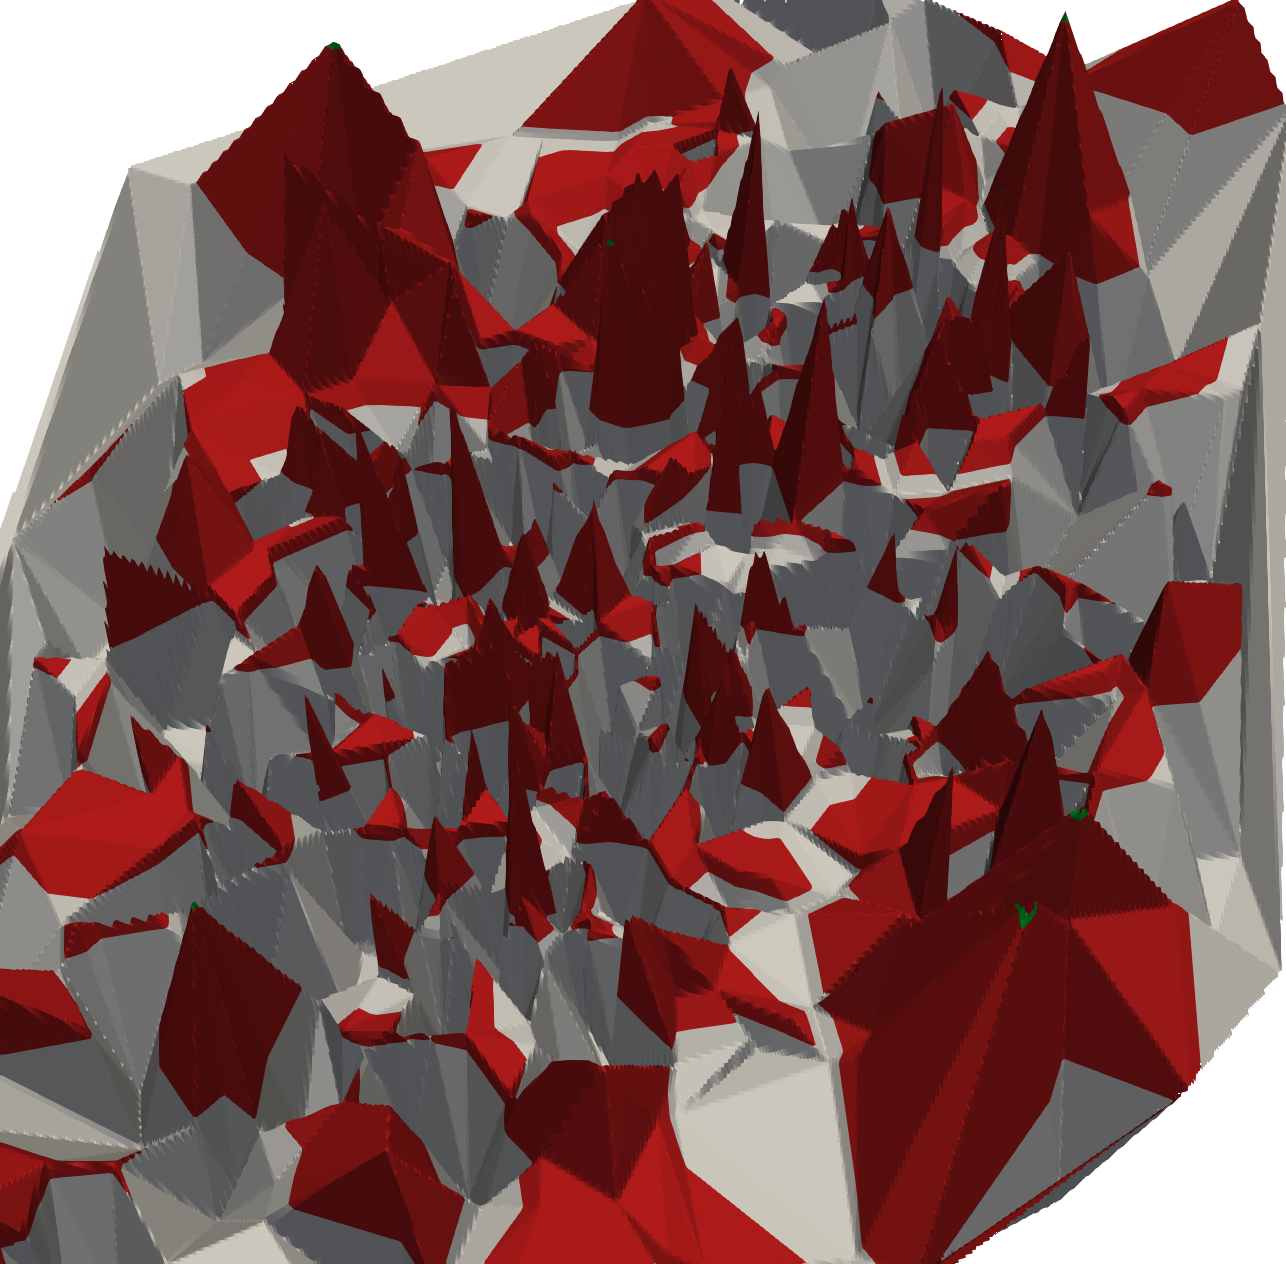
\includegraphics[width=\textwidth]{figures/coolidge-af-med-threshold.png}
		\caption{Med. threshold.}
		\label{fig:lvars-bench-overhead}
	\end{subfigure}
	~
	\begin{subfigure}[b]{0.33\textwidth}
    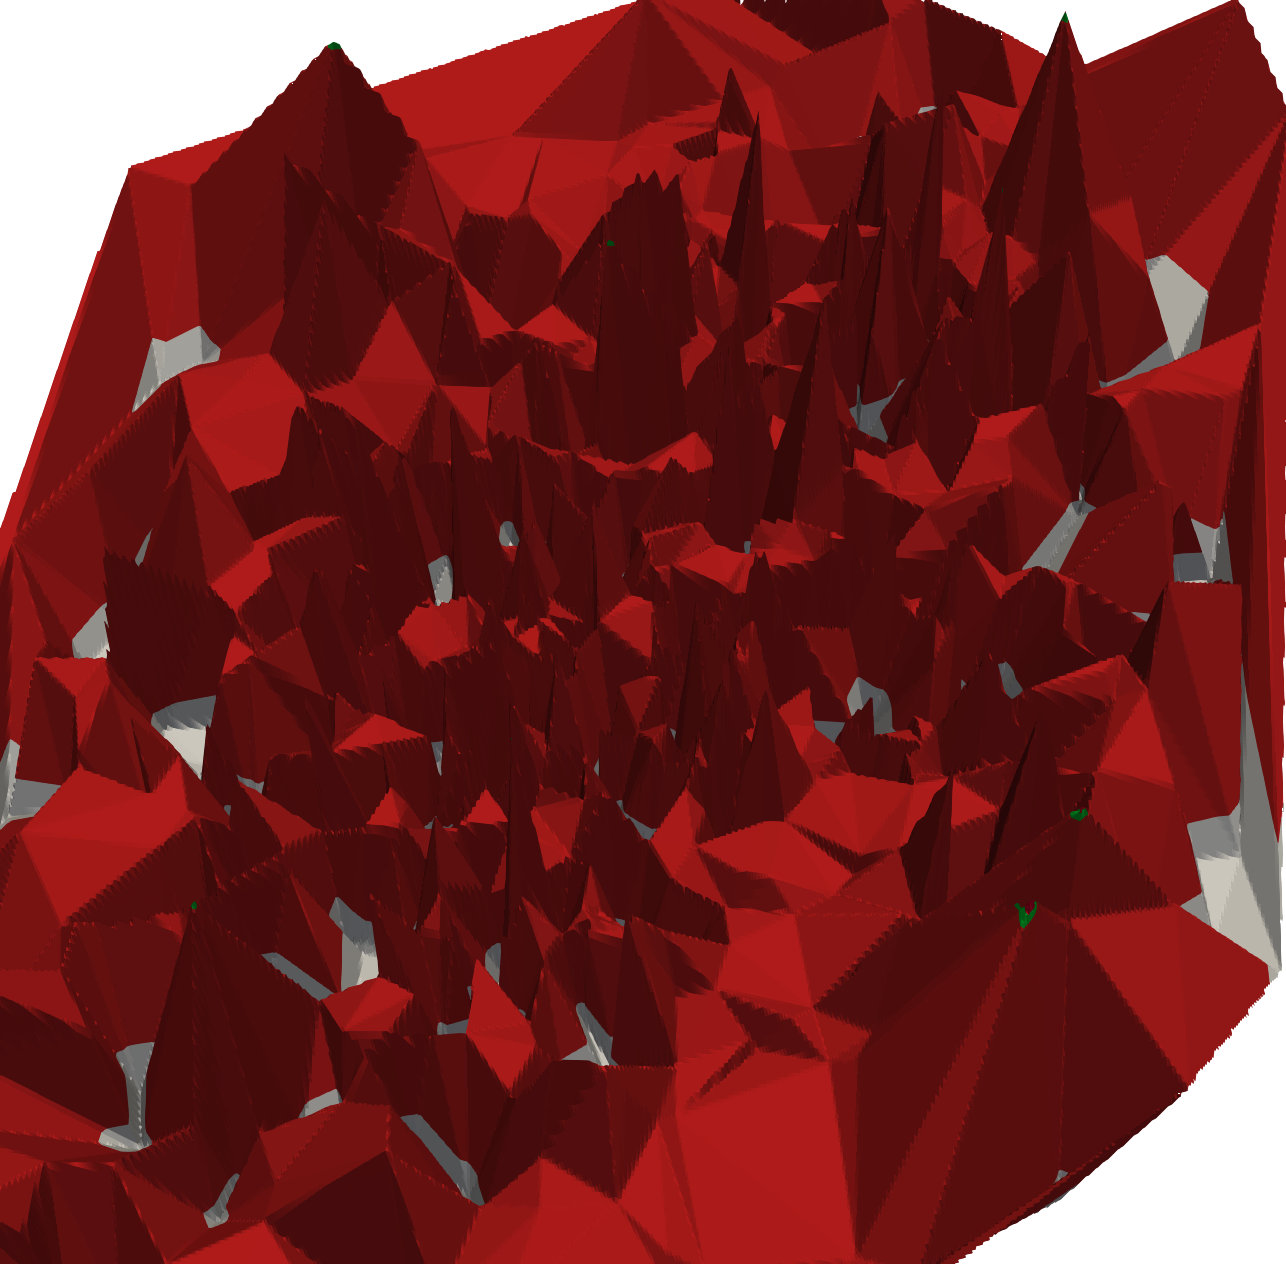
\includegraphics[width=\textwidth]{figures/coolidge-af-low-threshold.png}
		\caption{Low threshold.}
		\label{fig:lvars-bench-peak}
	\end{subfigure}

	\caption{Visualization of the design space for multiple thresholds}%
	\label{fig:visualization_design_centering_spaces}
\end{figure*}

Figure~\ref{fig:visualization_design_centering_spaces} again uses a visualization with the method described in~\cite{visualloss} to illustrate the intuition behind the design centering algorithm.
We see the mountain landscape of the mapping space, where the height is the execution time of that mapping.
The figure shows three different possible thresholds (high,medium,low). All peaks that are above the threshold are colored red: these depict infeasible points.
A robust mapping is a mapping such that we could ``walk'' in any direction from it without reaching one of the red peaks.
The larger the radius where this is possible, the more robust the mapping.
This metric interpretation of the design space allows us to use the metric-based algorithm of $L_p$ adaptation to estimate these neighborhoods around which we can walk without reaching a red peak.

The particular principle behind the $L_p$-adaptation algorithm is that it is based on estimating using an $L_p$ ball, i.e. with the $L_p$ norm $||x|| = (\sum_{i=1}^n x_i^p)^{1/p}$.
The algorithm is inspired on the evolution of robustness in biological systems~\cite{asmus2017lp}.
The basic principle behind the mapping is a two-step process, where simultaneously to the search for a design center, its robustness is estimated.
For the current candidate design center, uniformly random points from an $L_p$ ball around the point are sampled using an algorithm from~\cite{calafiore1998uniform}.
By assessing if these points are feasible, the algorithm can estimate the robustness of the design center.
In the next step thus, the algorithm adapts the design center and the estimated maximal radius.
Additionally, from the covariance matrix of the sampled points, the algorithm stores a linear transformation to skew or stretch the ball around a point.
This way, the neighborhoods are not restricted to balls $B_r(m)$ around the point $m$, but rather to linear transformations of such balls, i.e. $A B_r(m)$ for a matrix $A$ with $|\operatorname{det}(A)| = 1$.

\begin{figure}[h]
	\centering
   \resizebox{0.95\textwidth}{!}{\inputTikz{design_center_mapping_spaces.tex}}
	\caption{Examples of possible neighborhoods around design centers in two-dimensional random projections of the design space for the \texttt{audio filter} application on the Odroid XU4.}
	\label{fig:design_centering_exynos}
\end{figure}

These methods all rely on the metric space structure of the mapping space, as distances between mappings and the concept of neighborhoods all rely on the metric space structure.
Strictly speaking, neighborhoods can be defined on any topology, but not with radii as in the $L_p$ algorithm.
In~\cite{hempel_scopes17} we used the \texttt{SimpleVector} representation for this algorithm.
Here we also consider other metrics, as discussed in Section~\ref{sec:metric_spaces}.
In particular, we use the \texttt{MetricSpaceEmbedding} representation for mappings as discussed in~\cite{sec:representations}.
When considering other metrics, this also plays a role in the perturbation analysis.
In~\cite{hempel_scopes17} we define a perturbation to be a change in the mapping of exactly one process.\index{perturbations (of mappings)}
This is equivalent to a point with distance $1$ in the \texttt{SimpleVector} representation from the perturbed mapping.
Equivalently, if the change is uniformly at random, selecting such a point is equivalent to a uniformly random point in the ball $\overset{\circ}{B}_1(m) = B_1(m) \setminus \{ m \}$ without its center.
We can generalize this to use the distance metric in the used representation to perturb the points, selecting (uniformly) random points from the ball $B_r(m)$ in the corresponding representation.

To evaluate our methods, we re-implemented the $L_p$ adaptation algorithm and the corresponding perturbation tests in \mocasin. 
From a $1000$ random iterations we take the $1.,2.$ and $3.$ quartiles of the execution time for each of the three \texttt{CPN} applications on each platform, and we use those as thresholds to have a high, medium and low feasibility threshold level respectively.
We then execute the bio-inspired design centering flow with $10$ different random seeds for each of the threshold levels and compare centers to other (random) mappings for their stability using a perturbation test.

\begin{figure}[h]
	\centering
   \resizebox{0.95\textwidth}{!}{\inputTikz{design_centering_exynos.tex}}
	\caption{Design centering and perturbation stability for multiple threshold levels in the Odroid XU4 platform.}
	\label{fig:design_centering_exynos}
\end{figure}

Figure~\ref{fig:design_centering_exynos} shows the results of this method for mapping the \texttt{CPN} applications onto the Odroid XU4 platform.
We show the results for each application separately, for each of the three threshold levels. The thresholds are drawn onto the figure as horizontal dotted lines. 
This means that if after the perturbations mappings stay above the line, then the mapping is robust.
In almost all cases the design centering strategy indeed produces robust mappings, such that they are more robust than other (randomly chosen) points in a statistically significant manner.
For the Odroid XU4 platform we can see that the \texttt{MetricSpaceEmbedding} representation yields better results, albeit only slightly so.
We can see how this compares for the more complex platform, MPPA3 Coolidge.

\begin{figure}[h]
	\centering
   \resizebox{0.95\textwidth}{!}{\inputTikz{design_centering_coolidge.tex}}
	\caption{Design centering and perturbation stability for multiple threshold levels in the MPPA3 Coolidge platform.}
	\label{fig:design_centering_coolidge}
\end{figure}

Figure~\ref{fig:design_centering_coolidge} shows the results of the design centering via $L_p$ adaptation on the MPPA3 Coolidge.
In contrast to the simpler Odroid XU4, the \texttt{SimpleVector} representation yields clearly better results in this case.
Probably the so-called ``curse of dimensionality'' affects the algorithm here more, since it relies on traversing the hypervolume of the space, which is more difficult with a larger dimension.
Overall the $L_p$ algorithm seems to produce even more robust mappings in this case, yielding generally very good results.
A possible explanation for this is again the size of the design space.
In a larger space, with more points, it is plausible to also find larger neighborhoods of feasible points.

In this section we have successfully used metric space interpretations of the mapping space to adapt the $L_p$ adaptation algorithm to find robust mappings.
The mapping space, however, is a discrete space, while the $L_p$ adaptation assumes a continuous design space.
In the algorithm we deal with this problem by approximating a point to the closest mapping representing it.
However, a better strategy might be to adapt the $L_p$ adaptation algorithm itself to work on a discrete space.
This is a promising avenue for future work in this direction.